\documentclass{article}
\usepackage[english]{babel}
\usepackage[T1]{fontenc}
\usepackage{graphicx}
\usepackage[colorinlistoftodos]{todonotes}
\usepackage[colorlinks=true, allcolors=tudelftblue]{hyperref} %sets hyperlink colour
\usepackage{caption}
\usepackage{subcaption}
\usepackage{xcolor}
\usepackage{roboto} % for Roboto Slab font
\usepackage{float}
\usepackage{titling} 
\usepackage{blindtext}\usepackage{titlesec}
\usepackage[square,sort,comma,numbers]{natbib}
\usepackage[colorinlistoftodos]{todonotes}
\usepackage{tikz}
\usepackage{geometry}
\usepackage{sectsty}
\usepackage[utf8]{inputenc}
\usepackage{array}
\usepackage{makecell}
\usepackage{tabularx}
\usepackage{graphicx}
\usepackage[export]{adjustbox}
\usepackage{adjustbox}
\usepackage{amsmath}
\usepackage{tikzpagenodes}
\usepackage{booktabs}
\usepackage{listings}
\definecolor{tudelftdarkblue}{RGB}{0,0,0}
\definecolor{tudelftcyan}{RGB}{209,65,36}
\definecolor{tudelftblue}{RGB}{99, 102, 106}
\geometry{a4paper, margin=2cm}
\allsectionsfont{\color{black}} %sets colour for all headers
\usepackage{helvet}
\renewcommand{\familydefault}{\sfdefault}
\sectionfont{\fontfamily{RobotoSlab-TLF}\selectfont}
\setlength\parindent{0pt}
%%%%%%%%%%%%%%%%%%%%%%%%%%%%%%%%%%%%%%%%%%%%%%%%%%%%%%%%%
\begin{document}

\begin{titlepage}
    \fontfamily{RobotoSlab-TLF}\selectfont 
%%%%%%%%%%%%%%%%%%%%%%%%%%%%%%%%%%%%%%%%%%%%%%%%%%%%%%%%%%UNCOMMENT THE FOLLOWING FOR LESS "PLAIN" TITLE PAGE (SELECT WITH MOUSE AND PRESS CTRL AND /)

    % \begin{tikzpicture}[remember picture,overlay]
    %     % Set seed for random number generator
    %     \pgfmathsetseed{4}
    %     % Define the text area to avoid
    %     \path (current page text area.south west) rectangle (current page text area.north east);
    %     % Adding circles spread over the entire page
    %     \foreach \x in {1,...,1000}
    %         \draw[tudelftdarkblue] (current page.south west) ++(rand*\paperwidth,rand*\paperheight) circle (rand*0.3);
    %     % Define coordinates for the corners of the white box
    %     \coordinate (A) at ([shift={(-8cm,12cm)}]current page.center);
    %     \coordinate (B) at ([shift={(8cm,-5cm)}]current page.center);
    %     % Draw the white background box
    %     \fill[white] (A) rectangle (B);
    %     % Adding equations as background features
    %     \node[anchor=center,rotate=20,text=tudelftcyan] at ([shift={(-7cm,-2cm)}]current page.center) {\fontsize{18}{22}\selectfont
    %     $\nabla^2 T - \frac{1}{\alpha}\frac{\partial T}{\partial t} = 0$};
    %     \node[anchor=center,rotate=-15,text=tudelftcyan] at ([shift={(5cm,-4cm)}]current page.center) {\fontsize{18}{22}\selectfont
    %     $\frac{\partial \rho}{\partial t} + \nabla \cdot (\rho \mathbf{v}) = 0$};
    %     \node[anchor=center,rotate=20,text=tudelftcyan] at ([shift={(6cm,4cm)}]current page.center) {\fontsize{18}{22}\selectfont
    %     $a^2 + b^2 = c^2$};
    %     \node[anchor=center,rotate=10,text=tudelftcyan] at ([shift={(7cm,-2cm)}]current page.center) {\fontsize{18}{22}\selectfont
    %     $E = \frac{\sigma}{\varepsilon}$};
    %     \node[anchor=center,rotate=-10,text=tudelftcyan] at ([shift={(-6cm,4cm)}]current page.center) {\fontsize{18}{22}\selectfont
    %     $F = ma$};
    %     \node[anchor=center,rotate=5,text=tudelftcyan] at ([shift={(-4cm,-5cm)}]current page.center) {\fontsize{18}{22}\selectfont
    %     $Q = -\frac{kA}{\mu} \frac{\Delta P}{L}$};
    % \end{tikzpicture}
%%%%%%%%%%%%%%%%%%%%%%%%%%%%%%%%%%%%%%%%%%%%%%%%%%%%%%%%%%
    \vspace*{3cm}
    
    \centering
    {\Huge \textbf{\textcolor{black}{Festival della musica italiana}}}\\[1.5cm]
    \textsc{\LARGE Basi di Dati}\\[0.5cm]
    \text{\large The Bloodline}\\[2cm]
    
    {\Large \textbf{\textcolor{tudelftdarkblue}{Autori:}}}\\[0.5cm]
    \begin{tabular}{c}
        \Large \textcolor{tudelftdarkblue}{Aimen Omari (179980)} \\
        \Large \textcolor{tudelftdarkblue}{Ilir Alushi (176180)} \\
        
    \end{tabular}\\[2cm]
    
    
    
    \vfill
    \begin{center}
        
\includegraphics[width=0.6\textwidth]{images/Logo_C_Positivo_Colore.png}
    \end{center}
\end{titlepage}

%%% Create a table of contents
\tableofcontents


\newpage






\section{ANALISI DEI REQUISITI E VISTE}
In questo progetto presentiamo una base di dati che gestisce un festival musicale. \cite{Sanremo:1} Il festival avrà un sito web popolato da utenti che potranno svolgere varie attività e da amministratori che si occupano di gestire il sito. Inoltre, si occuperà di gestire le persone che parteciperanno al festival. 
Possiamo quindi considerare due classi di utente diverse:



\subsection{VISTA UTENTE ONLINE E SCHEMA SCHELETRO}
\textbf{\newline}
\textbf{VISTA UTENTE ONLINE}

\noindent\textbf{L'utente} è una classe di persona che è esclusivamente online. Sono caratterizzati da un nome, da un cognome, dall'età, dalla città di provenienza, dallo stato e dall'username che è unico. Essi son suddivisi a sua volta in utente base, utente abbonato e amministratore. Essi interagiscono attraverso il sito web. In primis possono cercare \textbf{gli artisti} partecipanti e consultare una serie di informazioni. Essi sono caratterizzati da un nome, da un cognome, dal genere musicale e dal nome d'arte che è univoco per ogni artista, inoltre possono essere identificati dal CF. Oltre a cercare informazioni sugli artisti possono cercare informazioni anche sull'\textbf{edizione} corrente come la località, il conduttore e come si svolgeranno le serate. Gli artisti portano un unico \textbf{brano} scelto da un album che devono portare in anteprima, accessibile solo dagli utenti abbonati. Esso è caratterizzato dal nome, univoco per ogni brano, dalla durata e dal genere. Ogni utente può assegnare un singolo \textbf{punteggio} per brano, che andrà da uno a dieci. Infine l'utente può creare liste che possono essere condivise in un forum. Una lista è caratterizzata dal nome, da un ID univoco e dagli artisti e brani inseriti. L'utente base ne può creare al massimo cinque. L'utente può sottoiscriversi ad un abbonamento ed esso gli garantisce specifiche aggiuntive. Oltre a ciò che fa l'utente base, l'utente abbonato può vedere la media dei punteggi per ogni brano. \cite{Rateyourmusic:2} Come detto prima, l'utente abbonato può accedere agli \textbf{album} in anteprima, caratterizzati dal nome e dal genere musicale. Esso può anche creare un numero illimitato di liste e cercare informazioni su edizioni passate. L'ultimo tipo di utente online, l'amministratore, ha le caratteristiche dell'utente base e sono coloro che si occupano di gestire il sito. Hanno il potere di modificare informazioni per ogni pagina web. Le pagine sono caratterizzate dal numero di pagina e contengono informazioni riguardanti gli artisti o l'edizione.
\newline

\noindent\textbf{GLOSSARIO DEI CONCETTI}

\begin{table}[h]
    \centering
    \begin{tabular}{|c|c|c|c|}
        \hline
          \textbf{Termine} & \textbf{Descrizione}  & \textbf{Sinonimo} & \textbf{Legame} \\
         \hline
         Utente & Nome, cognome, età, città, stato, username.  &  & Punteggio, pagine, liste, ricerca \\
         \hline
         Artista & Nome, cognome, CF, genere, nome d'arte  &  & Album \\
         \hline
         Brano&Nome, durata, genere &Canzoni  &Punteggio, album \\
         \hline
         Punteggio& Nome brano  &  &Utente, brano \\
         \hline
         Liste&Nome, ID  &  &Utente \\
         \hline
         Album&Nome, genere &  &Brano, artista \\
         \hline
         Pagine& Numero pagina  &  &Utente \\
         \hline
         Ricerca& Nome d'arte, ID festival &  & Utente \\
         \hline
    \end{tabular}
    \caption{Glossario dei concetti per la vista utente}
    \label{tab:glossario_utente}
    
\end{table}

\noindent\textbf{ELENCO OPERAZIONI UTENTE}
\begin{enumerate}
\item Può cercare informazioni sugli artisti partecipanti.
\item Può cercare informazioni sull'edizione corrente e su quelle passate.
\item Può valutare il brano di ogni artista.
\item Può creare liste composte da artisti o brani.
\item Può fare un abbonamento.
\item Può vedere la media dei punteggi assegnati al brano.
\item Può accedere all'anteprima degli album rilasciati dagli artisti.
\item Può modificare i dati delle pagine web del sito.
\end {enumerate}


\newpage
\noindent\textbf{SCHEMA SCHELETRO UTENTE}
\begin{figure}[h]
    \centering
    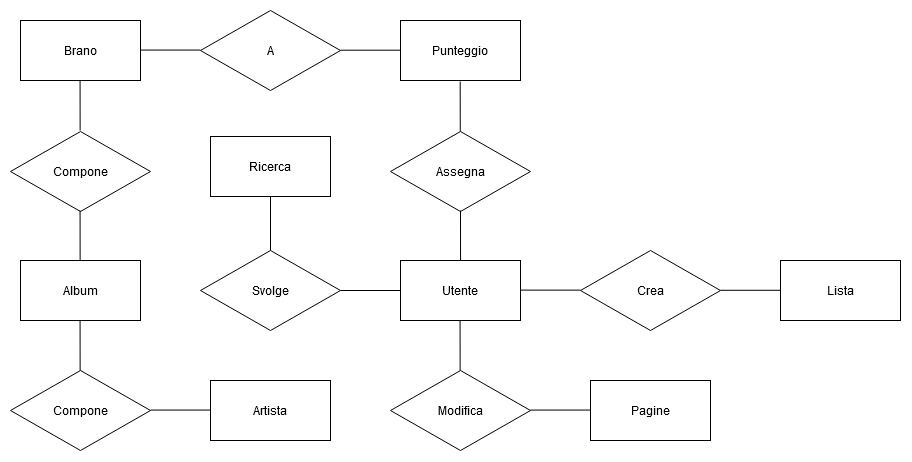
\includegraphics[width=1\linewidth]{images/Schema Scheletro Utente.jpg}
    \caption{Schema Scheletro Vista Utente}
    \label{fig:Vista Utente}
\end{figure}











\subsection{VISTA PERSONA FISICA E SCHEMA SCHELETRO}
\textbf{\newline}
\noindent\textbf{VISTA PERSONA}
\newline\newline
La \textbf{persona} è una classe di utente che sarà presente fisicamente nel festival. Sono caratterizzate da un nome, cognome e dal CF. Esse son suddivise a sua volta in spettatori, giuria e artisti. Gli artisti sono inoltre caratterizzati dal genere e dal loro nome d'arte. Essi hanno il compito di portare un album e da quell'album esporre una singola traccia al festival. Lo spettatore deve comprare un biglietto per accedere al festival tranne per un caso; se ha 7 anni o meno viene considerato spettatore giovane e può entrare gratis. Lo spettatore può anche vendere uno e un solo biglietto in un qualsiasi caso. Il \textbf{biglietto} è caratterizzato dal costo e dal codice biglietto che sarà univoco. Inoltre, come un utente, uno spettatore può valutare il brano caratterizzato dal nome, genere e dalla durata. Infine, può lasciare una mini \textbf{recensione} di massimo 50 parole per una singola traccia dopo l'ascolto. La giuria è un gruppo composto da pochi esperti che avrà il compito di giudicare da un ottica più critica ogni brano presentato al festival. Oltre al valutare i brani essi devono pubblicare una recensione per ogni brano. Le recensioni sono caratterizzate da un codice e per la giuria possono avere un massimo di 300 parole. Per ultimo dichiarano il \textbf{vincitore} del festival, esso è un artista e sarà scelto considerando la media dei punteggi tra utente, spettatore e giuria. Il vincitore verrà scelto una volta che tutti i membri della giuria hanno ascoltato e pubblicato una recensione per brano.
\newline
\newline
\textbf{GLOSSARIO DEI CONCETTI}

\begin{table}[h]
    \centering
    \begin{tabular}{|c|c|c|c|}
        \hline
         \textbf{Termine} & \textbf{Descrizione}  & \textbf{Sinonimo} & \textbf{Legame} \\
         \hline
         Persona & Nome, cognome, CF &  & Biglietti, recensioni, brani, vincitore \\
         \hline
      Biglietti&Codice, costo &  &Persona \\
         \hline
         Brani&Nome, genere, durata  &Traccia  &Persona, recensioni \\
         \hline
         Recensioni&Codice  &  &Persona, brani, album \\
         \hline
         Vincitore&Nome, cognome, genere, nome d'arte  &Artista  &Persona \\
         \hline
         Album&Nome, genere, artista  &  &Recensioni \\
         \hline
         Artista&Genere, nome d'arte &  &Vincitore \\
         \hline
    \end{tabular}
    \caption{Glossario dei concetti per la vista persona}
    \label{tab:my_label}
\end{table}

\newpage
\noindent\textbf{ELENCO OPERAZIONI PERSONA}
\begin{enumerate}
\item Può comprare biglietti.
\item Può vendere biglietti ad altre persone.
\item Può lasciare una recensione corta di 50 parole.
\item Può valutare il brano di ogni artista.
\item La giuria può fare una recensione di massimo 300 parole.
\item Possono scegliere il vincitore.
\newline\newline
\end {enumerate}

\noindent\textbf{SCHEMA SCHELETRO PERSONA}

\begin{figure}[h]
    \centering
    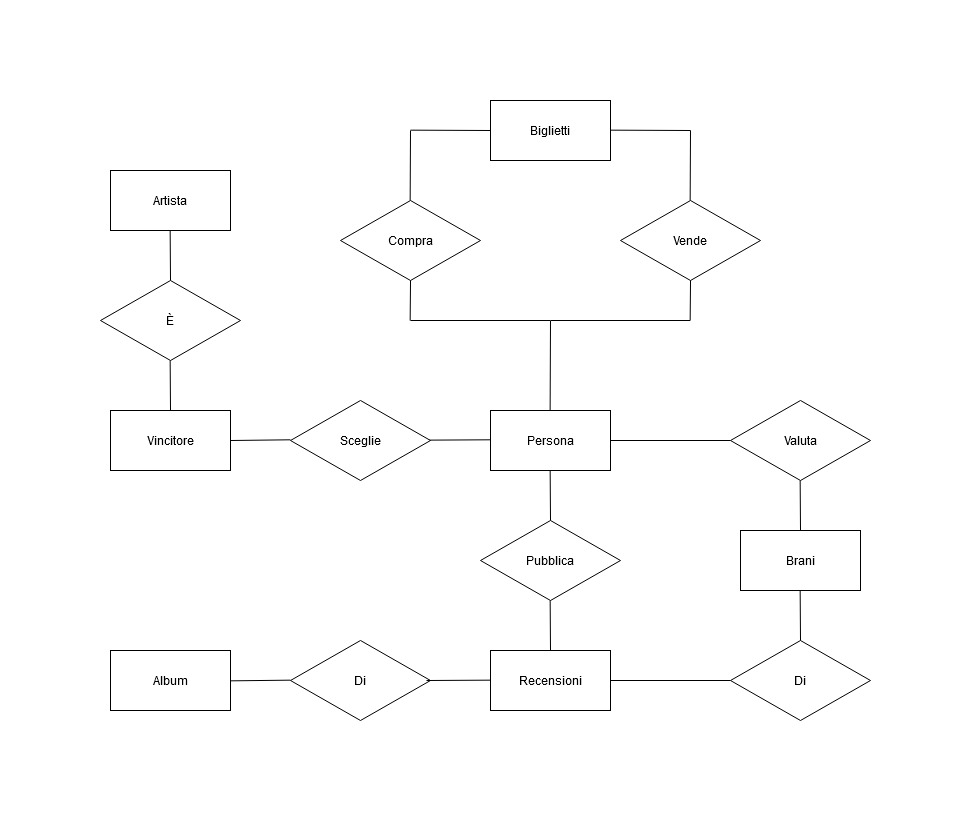
\includegraphics[width=1\linewidth]{images/Schema Scheletro Persona.jpg}
    \caption{Schema Scheletro Vista Persona}
    \label{fig:enter-label}
\end{figure}

\newpage

\section{SCHEMI ER}
\subsection{TRASFORMAZIONE VISTA UTENTE}
\noindent Per la vista dell'utente abbiamo iniziato generalizzando il concetto di Utente creando le entità Abbonato e Amministratore, che prenderanno come dati anagrafici nome, cognome, stato, città, età e l'username che è univoco per ogni utente. Per iniziare un utente assegna un punteggio ad un brano, che è stato modellato con una relazione con attributo voto. I brani comporranno album e a sua volta gli album sono composti da un artista, questo è stato espresso attraverso l'uso di identificatori esterni; un artista compone un album, gli album sono composti da più traccie e sarà unico il nome. Un utente inoltre è in grado di creare da 0 a 5 liste, cosa espressa con una relazione tra utente e lista. La modifica delle pagine sarà quindi assegnata all'amministratore, che gestirà le informazioni messe nelle varie pagine di artista e il brano oppure del festival. Oltre a ciò è possibile fare una ricerca per volta su un artista o su un festival e sulle sue edizioni passate, inoltre l'utente base può decidere di abbonarsi, l'abbonamento sarà unico e gli sarà possibile vedere il punteggio medio di ogni traccia ed accedere all'anteprima dei vari album.
\\
\\
\\
\\
\\
\\
\begin{figure}[h]
    \centering
    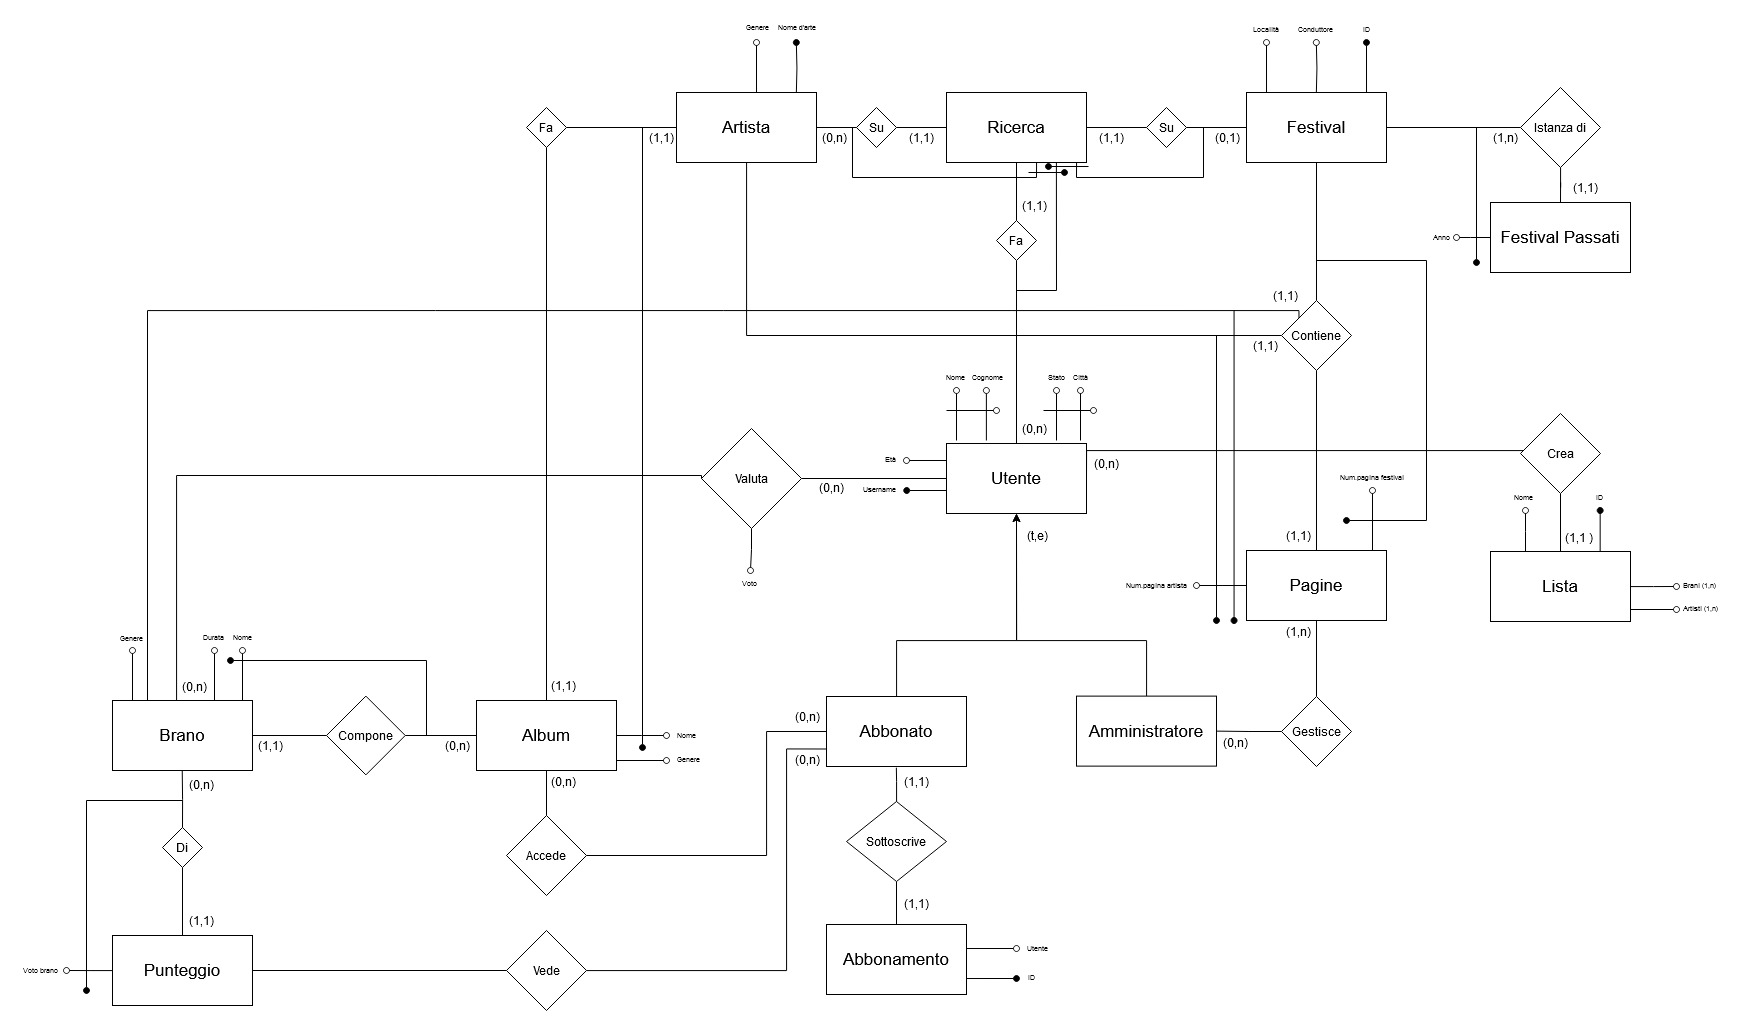
\includegraphics[max size={\textwidth}{\textheight}]{Vista Utente ER.jpg}
    \caption{Vista Utente ER}
    \label{fig:enter-label}
\end{figure}
\newpage
\subsection{TRASFORMAZIONE VISTA PERSONA}
\noindent
Per la vista della persona abbiamo iniziato generalizzando il concetto di Persona creando le entità Artista, Spettatore e Giuria. Essendo che sono tutte persone, abbiamo dato come attributi i vari dati anagrafici ed il CF, che riconoscerà univocamente ogni singola persona. In particolare per l'artista abbiamo aggiunto l'attributo nome d'arte che farà da chiave alternativa. Ci sarà una relazione con l'album dato che è lui che porta un album al festival. Dall'entità album abbiamo creato una relazione con l'entità brano, il brano è un appartenenza dell'album. Come attributi abbiamo scelto di mettere il nome e la durata e come chiave abbiamo preso la chiave primaria di album e l'abbiamo unita con l'attributo nome di brano. Per quanto riguarda lo spettatore, esso potrà eseguire molteplici operazioni, una tra le quali sarà vendere e acquistare biglietti, abbiamo creato una relazione con biglietto specificando che uno spettatore può acquistare/vendere più biglietti, può anche non venderli. Un biglietto può essere acquistato o venduto soltanto da una persona, inoltre esistono dei punti vendita da cui lo spettatore può acquistare biglietti e rivenderli a sua volta ad altri spettatori. Un'altra operazione che lo spettatore può fare è quella di valutare un brano e lasciare una recensione relativa all'album. Infine la giuria condivide una attività dello spettatore, ovvero recensire e valutare il brano scelto, inoltre potrà selezionare il vincitore del festival.
\begin{figure}[h]
    \centering
    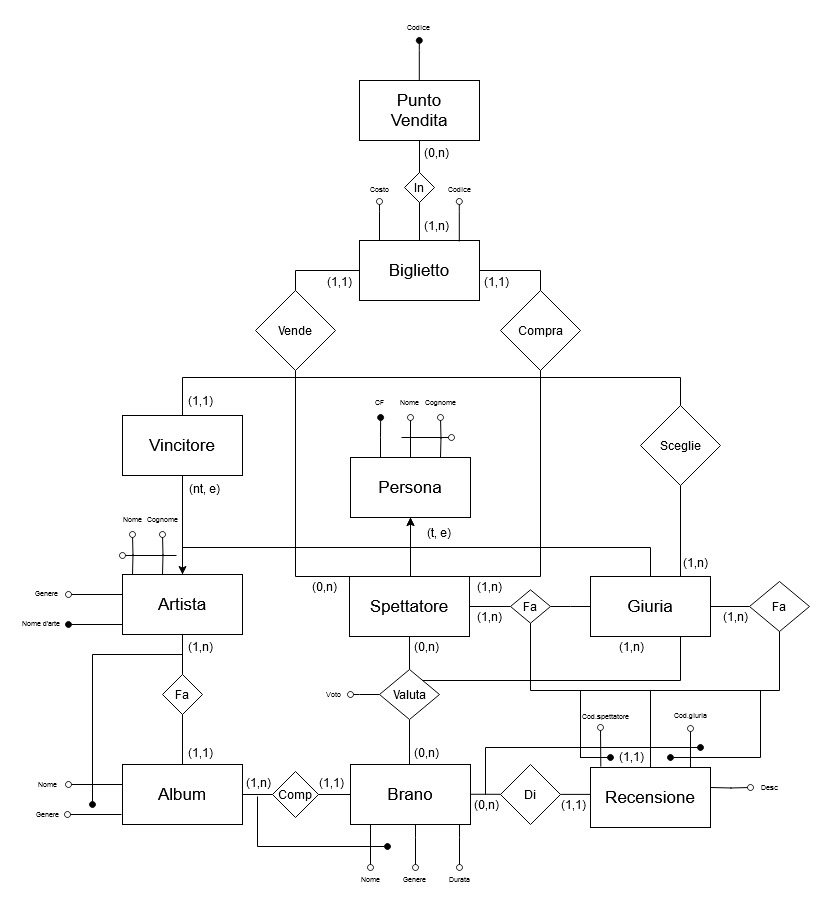
\includegraphics[width=0.9\linewidth]{Vista Persona ER.jpg}
    \caption{Vista Persona ER}
    \label{fig:enter-label}
\end{figure}
\newpage
\subsection{UNIONE DELLE VISTE IN UNICO E/R}
\noindent Questa è l'unione delle due viste.
\\
\\
\\
\\
\begin{figure}[h]
    \centering
    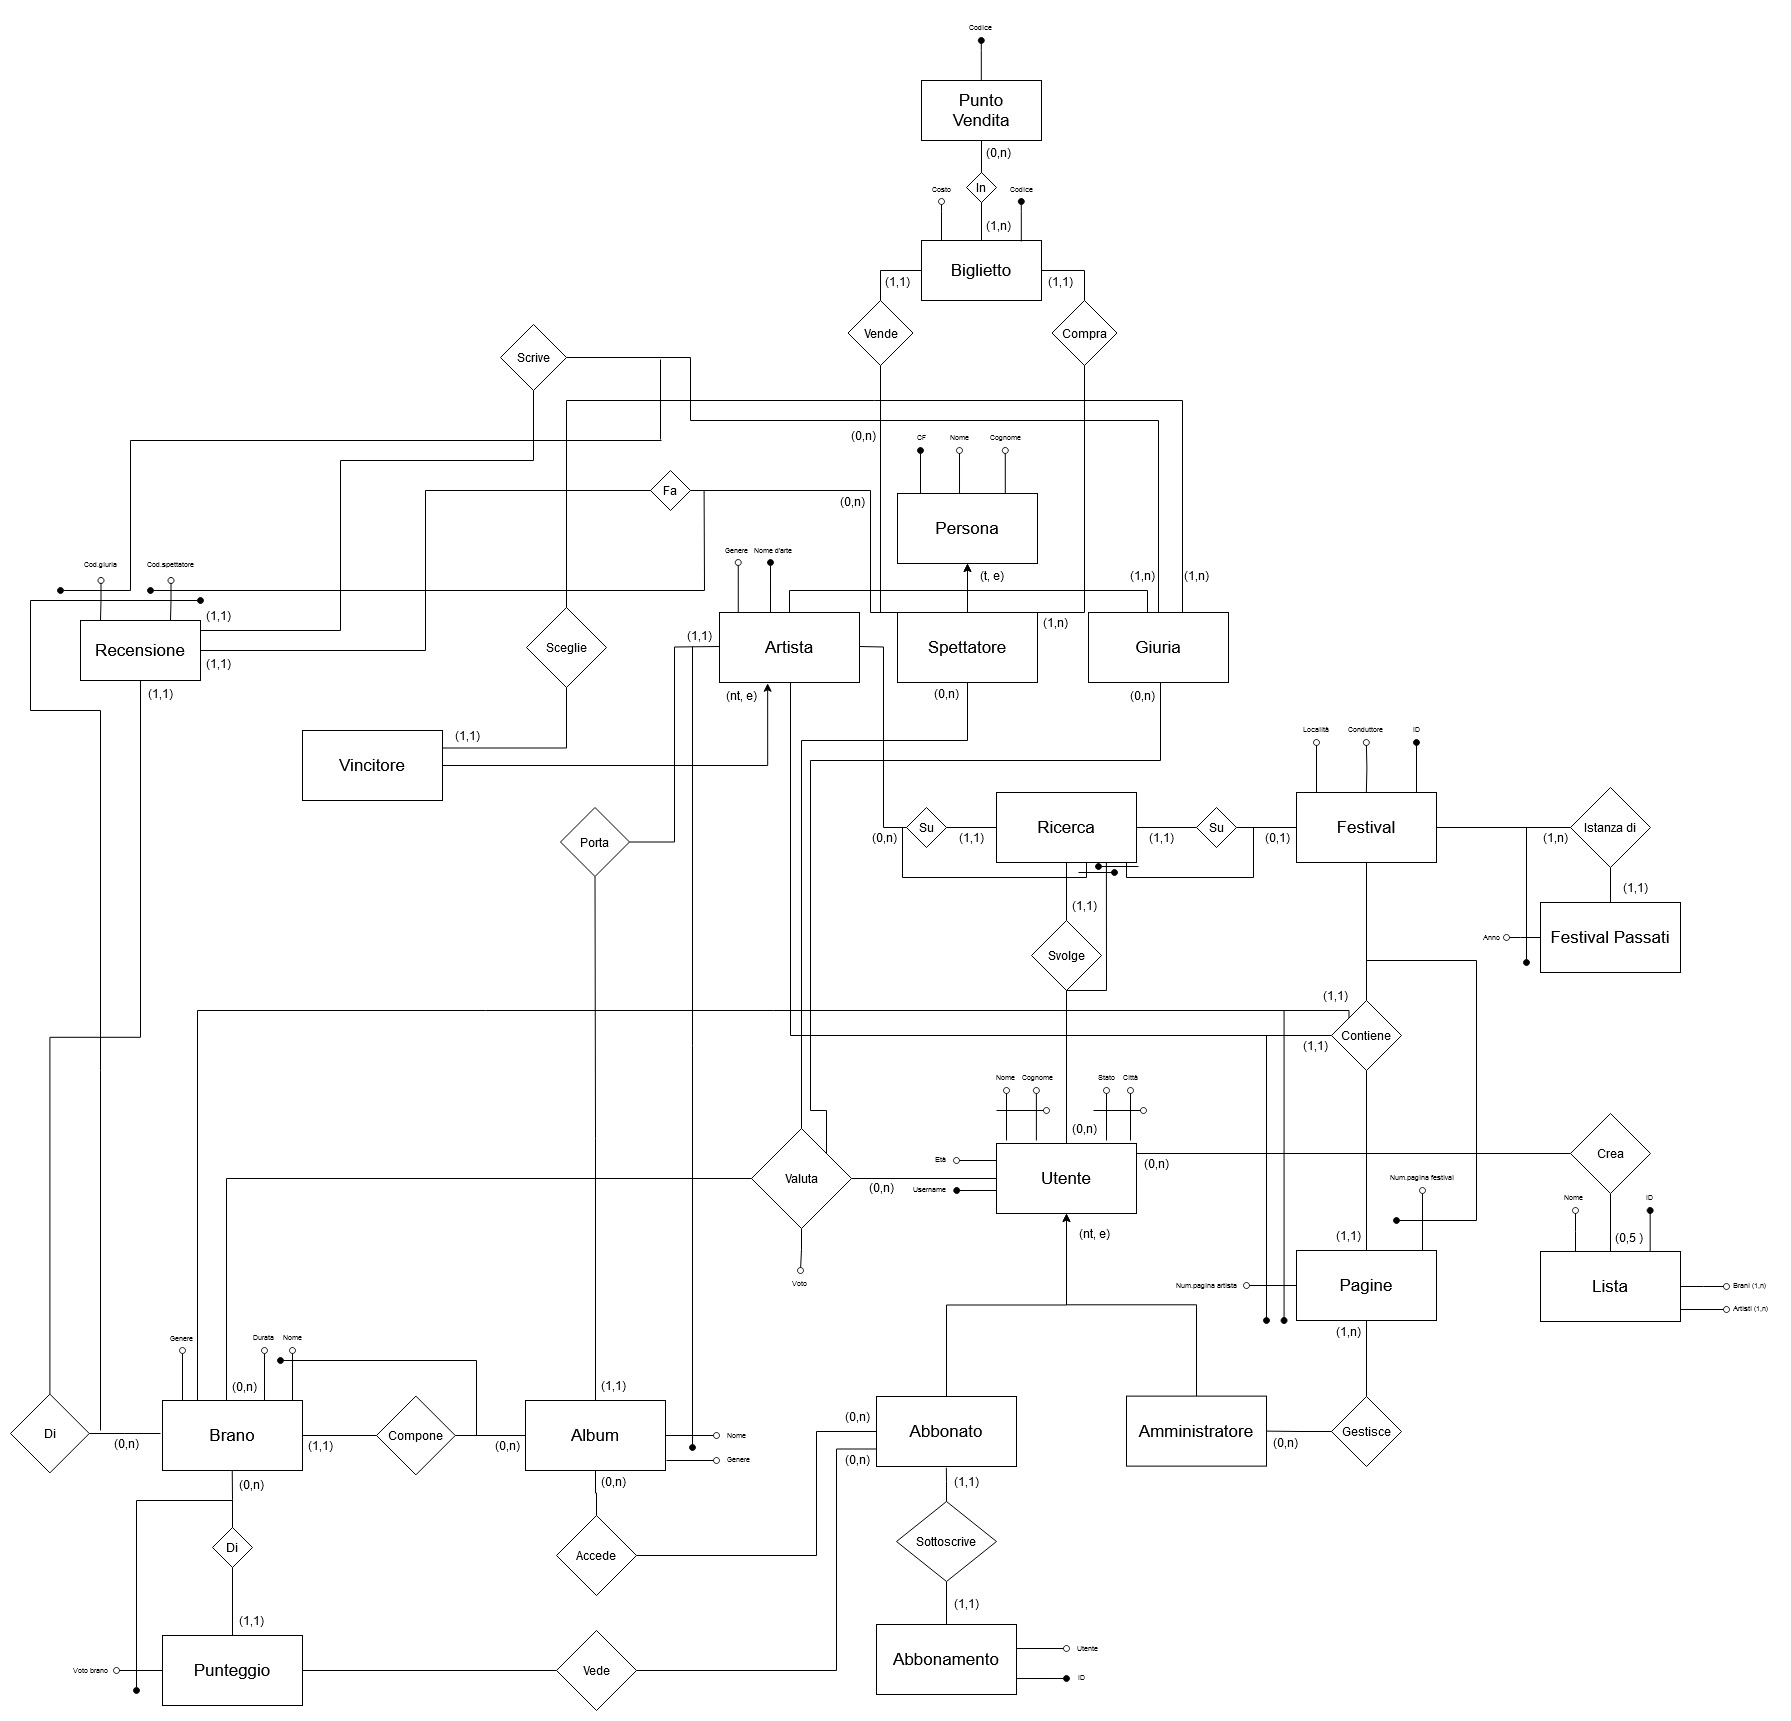
\includegraphics[max size={\textwidth}{\textheight}]{Vista Completa ER.jpg}
    \caption{Vista Completa ER}
    \label{fig:enter-label}
\end{figure}

\newpage
\subsection{DIZIONARIO DELLE ENTITA'}
\noindent Dizionario delle entità.
\\
\\
\\
\\

\begin{table}[ht]

    \centering
    \begin{adjustbox}{width=1.03\textwidth}
        \begin{tabular}{|p{2.5cm}|p{4.5cm}|p{5cm}|p{5cm}|}
            \hline
             \textbf{Entità}&\textbf{Descrizione}  &\textbf{Attributi}  &\textbf{Identificatore} \\
             \hline
             \makecell{Utente}&\makecell{Persona che interagisce con \\ il sito del festival}  &\makecell{Nome, cognome, stato \\ città, username}&\makecell{Username} \\
             \hline
             \makecell{Abbonato}&\makecell{Utente abbonato al sito} &\makecell{Nome, cognome, stato \\ città, età, username}  &\makecell{Username} \\
             \hline
             \makecell{Amministratore}&\makecell{Utente che gestisce il sito}  &\makecell{Nome, cognome, stato \\ città, età, username}  &\makecell{Username} \\
             \hline
             \makecell{Album}&\makecell{Una raccoltà di brani} &\makecell{Nome d'arte \\ genere, nome}&\makecell{Nome d'arte(FK)} \\
             \hline
             \makecell{Abbonamento}&\makecell{Ciò che l'utente svolge \\ per diventare abbonato}  &\makecell{Utente, ID} & \makecell{ID} \\
             \hline
             \makecell{Brano}&\makecell{Una canzone, \\ fa parte di un album}  &\makecell{Nome d'arte, nome.art \\ nome, durata, genere}&\makecell{(Nome d'arte \\ nome.art)(FK)} \\
             \hline
             \makecell{Punteggio}&\makecell{Un voto assegnato \\ ad un singolo brano}  &\makecell{Nome d'arte, nome.b \\ nome.art, voto brano}  &\makecell{(Nome.b, nome.art, \\ nome d'arte)(FK)} \\
             \hline
             \makecell{Festival}&\makecell{Il festival stesso}  &\makecell{ID, località \\ conduttore}  &\makecell{ID} \\
             \hline
             \makecell{Festival passati}&\makecell{Edizioni passate \\ del festival}  &\makecell{ID, anno}  &\makecell{ID(FK)} \\
             \hline
             \makecell{Artista}&\makecell{Si esibisce \\ al festival}  &\makecell{Nome d'arte} &\makecell{Nome d'arte}\\
             \hline
             \makecell{Lista}&\makecell{Una raccolta di \\ artisti o brani}  &\makecell{Nome, brani \\ artisti, ID}  &\makecell{ID} \\
             \hline
             \makecell{Pagina}&\makecell{Uno spazio che contiene \\ le informazioni \\ sugli artisti e sul festival}  &\makecell{N.pag, artista, \\ n.pag festival fest.ID, \\ b.nome, art.nome, nome d'arte}  &\makecell{Fest.ID(FK), Nome  d'arte(FK) \\ (art.nome, b.nome, \\ Nome d'arte)(FK)} \\
             \hline
             \makecell{Ricerca}&\makecell{Ricerca delle informazioni \\  del festival o dell'artista}  &\makecell{Username, \\nome d'arte, ID}  &\makecell{(Username, ID)(FK) \\ (Username, nome d'arte) (FK)} \\
             \hline
             \makecell{Persona}&\makecell{Persona che \\ partecipa al festival}  &\makecell{CF, Nome, \\Cognome}  &\makecell{CF} \\
             \hline
             \makecell{Spettatore}&\makecell{Guarda il festival}  &\makecell{CF, Nome, \\ Cognome}  &\makecell{CF} \\
             \hline
             \makecell{Giuria}&\makecell{Giudica i brani \\ del festival}  &\makecell{CF, Nome, \\ Cognome} & \makecell{CF}\\
             \hline
             \makecell{Recensione}&\makecell{Un commento \\ sul brano}  &\makecell{Cod.spett, \\cod.giuria, CF} &\makecell{(CF, cod.spettatore)(FK) \\ (CF, cod.giuria)(FK)} \\
             \hline
             \makecell{Biglietto}&\makecell{Ciò che compra lo spettatore \\ per accedere al festival}  &\makecell{Codice, costo}  &\makecell{Codice} \\
             \hline
             \makecell{Punto vendita}&\makecell{Dove si comprano \\ i biglietti}  &\makecell{Codice}  &\makecell{Codice} \\
             \hline
             \makecell{Vincitore}&\makecell{Vince il festival, \\ è un artista}  &\makecell{Nome d'arte, genere}  &\makecell{Nome d'arte} \\
             \hline
        \end{tabular}
         \end{adjustbox}
        \caption{Dizionario delle entità}
        \label{tab:my_label}
    \end{table}

\newpage    
\subsection{DIZIONARIO DELLE RELAZIONI}
\noindent Dizionario delle relazioni.
\\
\\
\\
\\

\begin{table}[ht]
    \centering
    \begin{adjustbox}{width=1\textwidth}
    \begin{tabular}{|p{2cm}|p{5cm}|p{5cm}|p{2.75cm}|}
        \hline
         \textbf{Relazioni}&\textbf{Descrizione}  &\textbf{Componenti}  &\textbf{Attributi} \\
         \hline
         \makecell{Sottoscrive}&\makecell{Abbonato che \\ sottoscrive un abbonamento}  &\makecell{Abbonato, abbonamento}  & \\
         \hline
         \makecell{Gestisce}&\makecell{Amministratori  \\ gestiscono delle pagine}  &\makecell{Amministratore, pagine}  & \\
         \hline
         \makecell{Contiene}&\makecell{Una pagina contiene \\ info sul festival o artisti}  &\makecell{Pagine, festival, \\ artista, brano}  & \\
         \hline
         \makecell{Crea}&\makecell{Gli utenti \\ possono creare liste}  &\makecell{Pagine, festival, \\ artista, brano}  & \\
         \hline 
         \makecell{Valuta}& \makecell{Gli utenti, gli spettatori e \\ la giuria possono valutare brani} &\makecell{Utente, brani, \\ spettatore, giuria}  &\makecell{Voto} \\
         \hline
         \makecell{Accede}&\makecell{Un utente abbonamento accede \\ agli album in anteprima}  &\makecell{Abbonato, album}  & \\
         \hline
         \makecell{Vede}&\makecell{Un abbonato vede \\ i punteggi degli album} &\makecell{Abbonato, brano}  & \\
         \hline
         \makecell{Compone}&\makecell{Ogni canzone è associata \\ ad un album. \\ In un album \\ sono associate più canzoni}  &\makecell{Album, Brano}  & \\
         \hline
         \makecell{Di}&\makecell{Una recensione viene \\ fatta su un brano } &\makecell{Brano, recensione}  & \\
         \hline
         \makecell{Svolge}&\makecell{Un utente svolge ricerche \\ per informarsi su festival e artisti} &\makecell{Utente, ricerca} & \\
         \hline
         \makecell{Porta}&\makecell{Un artista \\ porta un album}  &\makecell{Album, artista}  & \\
         \hline
         \makecell{Istanza di}& \makecell{Festival passato è \\ istance-of di festival} &\makecell{Festival passato, \\ festival} & \\
         \hline
         \makecell{Su}&\makecell{Una ricerca che \\ riguarda il festival} &\makecell{Ricerca, festival}  & \\
         \hline
         \makecell{Su}&\makecell{Una ricerca può \\ essere su un artista} &\makecell{Ricerca, artista} & \\
         \hline
         \makecell{Scrive}&\makecell{La giuria \\ scrive recensioni} &\makecell{Giuria, recensioni} & \\
         \hline
         \makecell{Fa}&\makecell{Uno spettatore può \\ scrivere una piccola recensione}  &\makecell{Spettatore, \\ recensione}  & \\
         \hline
         \makecell{Sceglie}&\makecell{La giuria sceglie \\ il vincitore}  &\makecell{Giuria, vincitore}  & \\
         \hline
         \makecell{Vende}&\makecell{Gli spettatori \\ possono vendere biglietti}  &\makecell{Spettatore, biglietto}  & \\
         \hline
         \makecell{Compra}&\makecell{Gli spettatori \\ possono comprare biglietti}  &\makecell{Spettatore, biglietto}  & \\
         \hline
         \makecell{In}&\makecell{I biglietti si comprano o \\vendono in punti vendita} &\makecell{Punto vendita, \\ biglietto}  & \\
         \hline
    \end{tabular}
    \end{adjustbox}
    \caption{Caption}
    \label{tab:my_label}
\end{table}

\newpage

\subsection{VINCOLI}

\noindent \textbf{VINCOLI NON ESPRIMIBILI DELLA VISTA UTENTE}
\begin{enumerate}
    \item Il punteggio potrà andare esclusivamente da zero a dieci.
    \item La lista dovrà riguardare solo brani oppure solo gli artisti.
    \item L'utente abbonato può creare infinite liste base.
    \item Solo l'utente abbonato può accedere ai festival passati.
    \item Le pagine possono contenere informazioni o sugli artisti o sul festival.
\end{enumerate}
\subsection{VINCOLI NON ESPRIMIBILI DELLA VISTA PERSONA}
\begin{enumerate}
    \item Se ha 7 anni o meno lo spettatore può entrare senza biglietto.
    \item La recensione degli spettatori può essere al massimo di 50 parole.
    \item La recensione della giuria può essere di massimo 300 parole.
    \item Il vincitore è scelto dalla media dei punteggi di giuria, spettatori e utente.
    Il punteggio della giuria vale di può rispetto agli altri due.
    \item Il vincitore verrà scelto una volta che tutti i membri della giuria hanno ascoltato e pubblicato una recensione per brano.
\end{enumerate}

\newpage
\section{SCHEMA LOGICO}
\noindent
\subsection{RISTRUTTURAZIONE DELLO SCHEMA E/R}
\begin{figure}[ht]
    \centering
    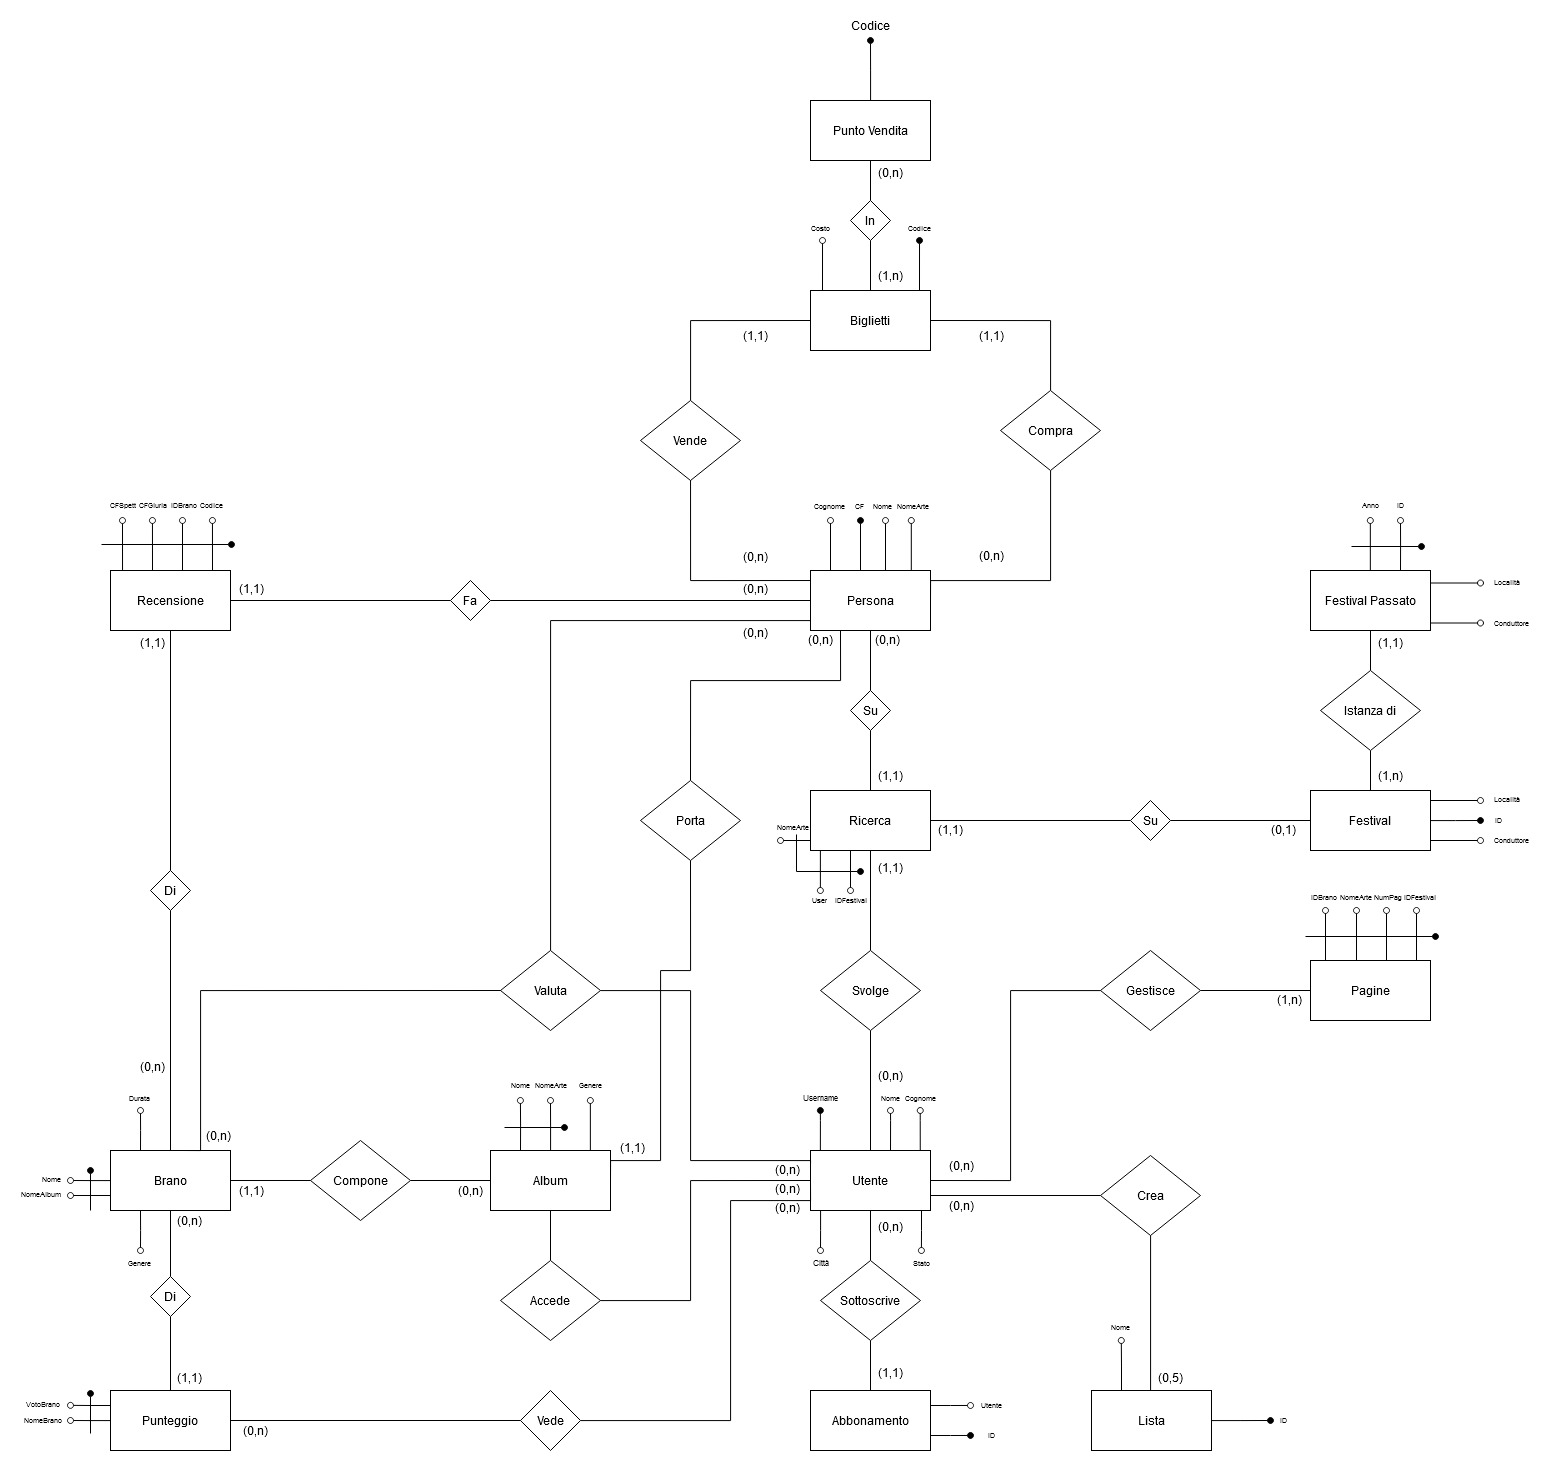
\includegraphics[width=1\linewidth]{Schema Logico.jpg}
    \caption{Ristrutturazione Schema ER}
    \label{fig:enter-label}
\end{figure}
\newpage
\subsection{TABELLA DEI VOLUMI E DELLE OPERAZIONI}
\begin{table}[ht]
    \centering
        \begin{tabular}{|p{3cm}|p{0.75cm}|p{3cm}|}
         \hline
         \textbf{Concetto}&\textbf{Tipo}  &\textbf{Volume dei dati} \\
         \hline
         
         Persona&E  &180000 \\
         \hline
         Biglietto&E  &180000 \\
         \hline
         Punto Vendita& E &200000 \\
         \hline
         Festival&E  &1 \\
         \hline
         Utente&E  &300000 \\
         \hline
         Valuta & R &100000 \\
         \hline
         Album&E  &30 \\
         \hline
         Sottoscrive&R  &30000 \\
         \hline
         Punteggio&E  &50000 \\
         \hline
         Lista&E  &120000 \\
         \hline
         Ricerca&E  &15000000 \\
         \hline
         Brano&E  &30 \\
         \hline
         Recensione&E  &90000 \\
         \hline
         Pagina&E  &40 \\
         \hline
    \end{tabular}
    \caption{Tabella dei volumi}
    \label{tab:my_label}
\end{table}

\begin{table}[ht]
    \centering
    \begin{tabular}{|p{5cm}|p{0.75cm}|p{3cm}|}
        \hline
         \textbf{Operazione}&\textbf{Tipo}  &\textbf{Frequenza} \\
         \hline
         Cercare info artisti&I  &180000/giorno \\
         \hline
         Cercare info edizione&I &31500/giorno \\
         \hline
         Valutare brano artista&I  &15000/giorno \\
         \hline
         Creare lista&I  &17500/giorno \\
         \hline
         Comprare abbonamento&I  &4250/giorno \\
         \hline
         Vedere media punteggi&I  &20000/giorno\\
         \hline
         Vedere anteprima album&I  &4250/giorno \\
         \hline
         Aggiungere/rimuovere dati&I  &500/giorno \\
         \hline
         Modificare dati&I  &250/giorno \\
         \hline
         Comprare biglietti&  I&25500/giorno \\
         \hline
         Vendere biglietti&I &2550/giorno \\
         \hline
         Lasciare recensione 50 parole&I  &8500/giorno \\
         \hline
         Lasciare recensione 300 parole&I  &42/giorno \\
         \hline
         Scegliere il vincitore&I  &1/settimana \\
         \hline
    \end{tabular}
    \caption{Tabella delle operazioni}
    \label{tab:my_label}
\end{table}
\newpage
\subsection{TABELLA DEI COSTI}


\begin{table}[ht]
    \centering
    \begin{tabular}{|p{2.5cm}|p{2.5cm}|p{2cm}|p{1.5cm}|}
        \hline
         \textbf{OPERAZIONE}&\textbf{CONCETTO}&\textbf{ACCESSO}  &\textbf{TIPO} \\
         \hline
         \makecell{OP1}& \makecell{\\PERSONA\\ COMPRA\\BIGLIETTI\\IN} &\makecell{1\\1\\1\\1}&\makecell{L\\S\\S\\S}\\
          \hline
          \makecell{OP2}&\makecell{PERSONA\\VENDE\\BIGLIETTO}  &\makecell{2\\1\\1}  &\makecell{L\\S\\S} \\
         \hline
         \makecell{OP3}&\makecell{FA\\RECENSIONE}  &\makecell{1\\1}  &\makecell{S\\S} \\
         \hline
         \makecell{OP4}&\makecell{PERSONA\\VALUTA}  &\makecell{1\\1}  &\makecell{L\\S} \\
         \hline
         \makecell{OP5}&\makecell{RECENSIONE\\FA} &\makecell{1\\1}  &\makecell{S\\S} \\
         \hline
    \end{tabular}
    \caption{Tabella costo operazioni persona}
    \label{tab:my_label}
\end{table}


\begin{table}[ht]
    \centering
    \begin{tabular}{|p{2.5cm}|p{3cm}|p{2cm}|p{1.5cm}|}
    \hline
         \textbf{OPERAZIONE}&\textbf{CONCETTO}  &\textbf{ACCESSO}  &\textbf{TIPO} \\
    \hline
    \makecell{OP1}&\makecell{RICERCA\\SVOLGE}  &\makecell{1\\1}  &\makecell{S\\S} \\
    \hline     
    \makecell{OP2}&\makecell{RICERCA\\SVOLGE\\SU\\FESTIVAL}  &\makecell{1\\1\\1\\1}  &\makecell{L\\L\\L\\L} \\
    \hline
    \makecell{OP3}&\makecell{UTENTE\\VALUTA\\BRANO}  &\makecell{1\\1\\1}  &\makecell{L\\S\\L} \\
    \hline
    \makecell{OP4}&\makecell{UTENTE\\CREA\\LISTE}  &\makecell{1\\1\\2.5}  &\makecell{L\\S\\S} \\
    \hline
    \makecell{OP5}&\makecell{UTENTE\\SOTTOSCRIVE\\ABBONAMENTO}  &\makecell{1\\1\\1} &\makecell{L\\S\\S} \\
    \hline
    \makecell{OP6}&\makecell{UTENTE\\VEDE\\PUNTEGGIO\\DI\\BRANO}  &\makecell{1\\50\\50\\50\\1}  &\makecell{L\\L\\L\\L\\L} \\
    \hline
    \makecell{OP7}&\makecell{UTENTE\\ACCEDE\\ALBUM}  &\makecell{1\\1\\1}  &\makecell{L\\L\\L} \\
    \hline
    \makecell{OP8}&\makecell{PAGINA\\PAGINA}  &\makecell{1\\1}  &\makecell{L\\L} \\
    \hline
    \end{tabular}
    \caption{Tabella costo operazioni utente}
    \label{tab:my_label}
\end{table}

\newpage
\subsection{TRADUZIONE DELLO SCHEMA E/R}

\noindent

Persona( \textbf{CF}, Nome, Cognome, Genere, NomeArtista)\\

Biglietto (\textbf{Codice}, Costo, CodicePV)\\
FK: CodicePV REFERENCES PuntoVendita
\newline

PuntoVendita(\textbf{Codice}, Nome)\\

Festival(\textbf{ID}, Conduttore, Località)\\

FestivalPassato(\textbf{ID, Anno}, Conduttore, FestivalID)\\
FK: ID REFERENCES Festival\\

Utente (\textbf{Username}, Nome, Cognome, Stato, Città)\\

Valuta (\textbf{Username, Nome}, Voto)\newline
FK: Username REFERENCES Utente\\
FK: Nome REFERENCES Brano\\

Album (\textbf{Nome}, Genere, \textbf{NomeArtista})\newline
FK: NomeArtista REFERENCES Persona\\

Sottoscrive (\textbf{Username}, \textbf{IDAbbonamento}) \\
FK: Username REFERENCES Utente\newline
FK: IDAbbonamento REFERENCES Abbonamento\newline

Punteggio (\textbf{VotoBrano}, \textbf{NomeBrano})\newline
FK: NomeBrano REFERENCES Brano\\

Lista (\textbf{Username}, \textbf{ID}, Nome)\newline
FK: Username REFERENCES Utente\\

Ricerca (\textbf{IDFestival}, NomeDArte, \textbf{IDUtente}) \newline
FK: IDUtente REFERENCES Utente\\
FK: IDFestival REFERENCES Festival\\
FK: NomeDArte REFERENCES Persona \\

Recensione (\textbf{CodiceGiuria}, \textbf{CodiceSpettatore}, IDBrano)\\
FK: IDBrano REFERENCES Brano \\
FK: CodiceGiuria REFERENCES Giuria\\
FK: CodiceSpettatore REFERENCES Persona\\

Pagina (\textbf{NPagArtista}, \textbf{IDFestival}, \textbf{NomeDArte}, \textbf{IDBrano} )
\\
FK: IDFestival REFERENCES Festival\\
FK: NomeDArte REFERENCES Persona\\
FK: IDBrano REFERENCES Brano\\

Brano(\textbf{ID}, \textbf{Nome, NomeAlbum}, Genere, Durata)\\
FK: NomeAlbum REFERENCES Album \\

Abbonamento(\textbf{ID}, NomeAbbonamento, Costo)\\
FK: NomeAbbonamento REFERENCES Utente \\

Spettatore(\textbf{CF}, Nome, Cognome, Età, NomeArtista) \\
FK: CF REFERENCES Persona \\

Giuria(\textbf{Codice}, NumGiudici)


\newpage
\section{INDICI}
\subsection{Performance degli Indici}

Indice per ottimizzare le query che ordinano Album: \\
\textbf{CREATE INDEX} idx\_album\_nomedarte \textbf{ON} Album (NomeDArte)
\\

Indice per ottimizzare le query ordinano Artisti: \\
\textbf{CREATE INDEX} idx\_persona\_nomeartista \textbf{ON} Persona (NomeArtista)
\\

Indice per ottimizzare le query ordinano Brani: \\
\textbf{CREATE INDEX} idx\_brano\_nome \textbf{ON} Brano (Nome)
\\
\\
\\

\textbf{TEST QUERY:} \\
\\
1) Trova gli artisti che hanno un brano con un voto medio superiore alla media di tutti i brani: \\ \\
\textbf{PRE-INDICI:} Planning Time: 0.244ms - Execution Time: 4561.427ms \\
\textbf{POST-INDICI:} Planning Time: 0.327ms - Execution Time: 20.283ms \\

2) Trova i brani che hanno una media di voti superiore a 4, insieme alle informazioni sugli album e gli artisti \\ \\
\textbf{PRE-INDICI:} Planning Time: 0.330ms - Execution Time: 5.951ms \\
\textbf{POST-INDICI:} Planning Time: 0.241ms - Execution Time: 0.117ms \\

\newpage
\section{BIBLIOGRAFIA}

\bibliographystyle{apalike}
\bibliography{ref}

\end{document}


%All other official TU Delft colours
\definecolor{donkerblauw}{RGB}{12, 35, 64}
\definecolor{turkoois}{RGB}{0, 184, 200}
\definecolor{blauw}{RGB}{0, 118, 194}
\definecolor{paars}{RGB}{111, 29, 119}
\definecolor{roze}{RGB}{239, 96, 163}
\definecolor{framboos}{RGB}{165, 0, 52}
\definecolor{rood}{RGB}{224, 60, 49}
\definecolor{oranje}{RGB}{237, 104, 66}
\definecolor{geel}{RGB}{255, 184, 28}
\definecolor{lichtgroen}{RGB}{108, 194, 74}
\definecolor{donkergroen}{RGB}{0, 155, 119}
%You can use these to change the hyperlink colour or the colour of the header or whatever. Glück Auf!